%%%%%%%%%%%%%%%%%%%%%%%%%%%%%%%%%%%%%%%%%%%%%%%%%%%%%%%%%%%%%%%%%%%%%%%%%%%%%%%%
%                                   PREAMBLE                                   %
%%%%%%%%%%%%%%%%%%%%%%%%%%%%%%%%%%%%%%%%%%%%%%%%%%%%%%%%%%%%%%%%%%%%%%%%%%%%%%%%

% Compile with 'latexmk -shell-escape -pdf guide'.

%%%% DOCUMENT CLASS %%%%%%%%%%%%%%%%%%%%%%%%%%%%%%%%%%%%%%%%%%%%%%%%%%%%%%%%%%%%

% Global options declared here may be used by packages below. For example:
%
% 1. Language options, like 'english' or 'spanish', are used by package 'babel'.
% 2. Paper size options, like 'a4paper', are used by package 'geometry'.
%
% Options like 'american', 'british', 'canadian', 'australian', 'newzealand'
% represent variants of English.

\documentclass[british,a4paper,11pt,titlepage]{article}

%%%% FONT ENCODING %%%%%%%%%%%%%%%%%%%%%%%%%%%%%%%%%%%%%%%%%%%%%%%%%%%%%%%%%%%%%

% T1 is an 8-bit encoding for a set of 256 glyphs, the standard LaTeX glyph set
% that covers most European languages that use Latin alphabets.

\usepackage[T1]{fontenc}        % T1 font encoding.

%%%% FONTS %%%%%%%%%%%%%%%%%%%%%%%%%%%%%%%%%%%%%%%%%%%%%%%%%%%%%%%%%%%%%%%%%%%%%

% Fonts should match the specified font encoding. There are different packages
% providing different fonts with different encodings.

\usepackage{lmodern}            % Translation of Computer Modern into T1 fonts.

% Alternative T1 fonts based on the Adobe Utopia fonts:
%
% Utopia Regular, Utopia Italic, Utopia Bold, and Utopia Bold Italic
%
% \usepackage{fourier}
%
% Alternative T1 fonts containing the whole LaTeX glyph set and matching fonts
% for mathematics:
%
% https://www.ctan.org/pkg/mathdesign
%
% \usepackage[utopia]{mathdesign}
% \usepackage[garamond]{mathdesign}
% \usepackage[charter]{mathdesign}

% Font selection is greatly simplified with XeLaTeX and LuaLaTeX, particularly
% thanks to the use of Unicode and support for Apple Advanced Typography (AAT),
% TrueType (TTF) and OpenType (OTF) fonts through the fontspec package (other
% relevant packages include unicode-math, mathspec, and fontsetup).
%
% A catalogue of free fonts can be found here:
%
% https://tug.org/FontCatalogue

%%%% INPUT ENCODING %%%%%%%%%%%%%%%%%%%%%%%%%%%%%%%%%%%%%%%%%%%%%%%%%%%%%%%%%%%%

% The selected encoding must match the encoding the file is written. For
% example, if you are using a Unicode text editor and saving your documents with
% the typical UTF-8 encoding, you should use the following:

\usepackage[utf8]{inputenc}

% In fact, this is the default input encoding in recent versions, so you can
% omit this, though it will not hurt.

% Unicode character recognition: https://shapecatcher.com
% LaTeX symbol recognition:      https://detexify.kirelabs.org

% Other usual encodings:

% \usepackage[latin1]{inputenc}   % ISO 8859-1 encoding.
% \usepackage[latin9]{inputenc}   % ISO 8859-15 encoding (includes the € sign).

%%%% PAGE FORMAT %%%%%%%%%%%%%%%%%%%%%%%%%%%%%%%%%%%%%%%%%%%%%%%%%%%%%%%%%%%%%%%

% Page geometry, margins, etc.

\usepackage{geometry}

% Empty pages really empty, without page numbers and headings.

\usepackage{emptypage}

% Paragraphs without indentation and separated by vertical space.

\usepackage[parfill]{parskip}

% PDF metadata, hyperlinks, and bookmarks.

\usepackage[pdfusetitle,colorlinks,citecolor=magenta,linkcolor=blue]{hyperref}

% Improved bookmarks.

\usepackage{bookmark}

% Author blocks (name and affiliation).

\usepackage[auth-sc,blocks]{authblk}

% We found a problem here! Unfortunately, package 'authblk' interferes with the
% inner mechanism by which 'hyperref' provides author metadata (pdfauthor)
% thanks to the option 'pdfusetitle'. As a consequence, author metadata in the
% PDF remains empty. However, we are fortunate, because LaTeX is free,
% open-source, programmable and well-documented. The same with these LaTeX
% packages. No wonder we could study the package documentation (and even the
% source code when necessary) and patch the definition of the '\author' macro to
% fix it. Even better. We were able to find an almost working solution in the
% Internet (TeX Stack Exchange).

\usepackage{xpatch}             % Patching facilities.

\xpretocmd{\author}{\addauthor{#2}}{}{}

\newif\iffirstauthor            % New 'if'.
\firstauthortrue                % Initially, true.

\newcommand{\addauthor}[1]
{
    \iffirstauthor                  % First author?
    \newcommand{\hrauthor}{#1}    % The author name.
    \firstauthorfalse
    \else                           % Other authors?
    \xapptocmd{\hrauthor}{, #1}{}{} % A comma followed by the author name.
    \fi
}

%%%% BIBLIOGRAPHY %%%%%%%%%%%%%%%%%%%%%%%%%%%%%%%%%%%%%%%%%%%%%%%%%%%%%%%%%%%%%%

% The modern and powerful BibLaTeX, with the default Biber back-end (option
% 'backend=biber' is set by default).

\usepackage{csquotes}           % Context-sensitive quotations.
\usepackage{biblatex}

% Changing the style.

% Numeric (the default style), in citation order, with back-references.

% \usepackage[style=numeric,sorting=none,backref]{biblatex}

% Author-year, sorted by name-year-volume-title.

% \usepackage[style=authoryear,sorting=nyvt,block=space,backref]{biblatex}

% It is possible to mix styles (the combination should be sensible so that it
% does not hamper search in a printed copy). For example, author-year for
% citations and author-title for bibliography items.

% \usepackage[citestyle=authoryear,bibstyle=authortitle,block=ragged]{biblatex}

% Redefining the URL field (break the line before and turn the space after the
% colon into a non-breaking space

\DeclareFieldFormat{url}{\newline\mkbibacro{URL}\addcolon\nobreakspace\url{#1}}

\addbibresource{references.bib}

%%%% MATHEMATICS %%%%%%%%%%%%%%%%%%%%%%%%%%%%%%%%%%%%%%%%%%%%%%%%%%%%%%%%%%%%%%%

% AMS mathematical delicatessen.

\usepackage{amsmath}
\usepackage{amssymb}
\usepackage{amsthm}

%%%% FIGURES AND TABLES %%%%%%%%%%%%%%%%%%%%%%%%%%%%%%%%%%%%%%%%%%%%%%%%%%%%%%%%

% Publication-quality tables.

\usepackage{array,booktabs}

% Captions for subfigures and subtables.
%
% This is an alternative to package subfig. Please, notice that package
% subfigure, which is superseded by subfig, is obsolete and deprecated.

\usepackage{subcaption}

% Enhanced support for the inclusion of external graphics.

\usepackage{graphicx}

% Plots and tables with TikZ & PGF.

\usepackage{pgfplotstable}

\usetikzlibrary{intersections}

%%%% CODE AND PSEUDO CODE FORMATTING %%%%%%%%%%%%%%%%%%%%%%%%%%%%%%%%%%%%%%%%%%%

% Improved verbatim text.

% \usepackage{verbatim}

% Much improved, and configurable, verbatim text.

% \usepackage{fancyvrb}

% Source code listing with basic syntax highlighting.

% \usepackage{listings}

% Syntax highlighting through Python's Pygments library.
%
% apt install python-pygments
%
% Please, notice that '-shell-escape' will be required when compiling to
% execute the necessary external commands.

\usepackage[cachedir=.minted-\jobname]{minted}

%%%% ATTACHMENTS %%%%%%%%%%%%%%%%%%%%%%%%%%%%%%%%%%%%%%%%%%%%%%%%%%%%%%%%%%%%%%%

% Attach source files to the output PDF document.

\usepackage{embedfile}

\embedfile{references.bib}
\embedfile{coloreado_grafos.png}
\embedfile{normales.png}
\embedfile{normales_log.png}
\embedfile{optimizado.png}
\embedfile{optimizado_log.png}

%%%% MISCELLANY %%%%%%%%%%%%%%%%%%%%%%%%%%%%%%%%%%%%%%%%%%%%%%%%%%%%%%%%%%%%%%%%

% To-do notes.

\usepackage[backgroundcolor=red!10,bordercolor=white,shadow]{todonotes}

% Logos for TeX and derivatives.

\usepackage{metalogo}

% Expert typographical adjustments.

\usepackage{microtype}

% A package for purists: it warns about the use of obsolete LaTeX features.

% \usepackage[l2tabu,orthodox]{nag}

%%%% LOCALISATION AND INTERNATIONALISATION %%%%%%%%%%%%%%%%%%%%%%%%%%%%%%%%%%%%%

% Babel provides automatic customisation of many cultural and language-related
% features depending on the language specified.

\usepackage{babel}

%%%% USER-DEFINED COMMANDS AND ENVIRONMENTS %%%%%%%%%%%%%%%%%%%%%%%%%%%%%%%%%%%%

% We can redefine some commands to reflect a particular writing style or define
% new ones, thus providing content markup to separate presentation from content.

% Content markup for a matrix.

\newcommand{\mat}[1]{#1}        % No presentation markup inside in this case.

% Now, we can consider changes in presentation. For example, ISO 80000-2:2019
% mandates boldface for vectors and matrices, and boldface sans serif for
% tensors, though an arrow above the letter symbol is allowed instead of
% boldface to indicate a vector (and two arrows instead of boldface sans serif
% for tensors).

% Vectors are already provided by command '\vec' in package 'amsmath', which
% presents them in arrow notation. We redefine the command to present them in
% boldface instead.

% \renewcommand{\vec}[1]{\boldsymbol{#1}}

% Then, we redefine our previously defined '\mat' command to present matrices in
% boldface, analogously to '\vec'.

% \renewcommand{\mat}[1]{\boldsymbol{#1}}

% Additional examples follow.

% Uppercase and lowercase Greek letter omicron in the default mathematical style.

\newcommand{\Omicron}{\mathrm{O}} % Upright, same glyph that Latin O.
\newcommand{\omicron}{\mathit{o}} % Slanted, same glyph that Latin o.

% File name.

\newcommand{\file}[1]{\url{#1}}

% This is a bit different alternative, as 'file://' is added to the path.

% \newcommand{\file}[1]{\href{file://#1}{\texttt{#1}}}

% Tool name (e.g., PDFLaTeX).

\newcommand{\tool}[1]{\emph{#1}}

% Command name (e.g., pdflatex).

\newcommand{\command}[1]{\texttt{#1}}

% E-mail address (hyperlinked).

\newcommand{\email}[1]{\href{mailto:#1}{\textsf{#1}}}

% C++, as typeset in the C++ standard.

\usepackage{relsize}            % We will use '\smaller' next.

\newcommand{\plus}{\protect\hspace{-.1em}\protect\raisebox{.35ex}{\smaller{\smaller\textbf{+}}}}
\newcommand{\CPP}{\mbox{C\plus\plus}}

%%%%%%%%%%%%%%%%%%%%%%%%%%%%%%%%%%%%%%%%%%%%%%%%%%%%%%%%%%%%%%%%%%%%%%%%%%%%%%%%
%                                 FRONT MATTER                                 %
%%%%%%%%%%%%%%%%%%%%%%%%%%%%%%%%%%%%%%%%%%%%%%%%%%%%%%%%%%%%%%%%%%%%%%%%%%%%%%%%

\newrefsegment                  % Begin collecting references cited (segment 1).

\begin{document}

% The following command is defined if your document class is 'book'.
%
% It switches to Roman numerals for page numbering and omit numbers in chapter
% titles (as with the starred sectioning command \chapter*), though chapter
% titles will appear in the table of contents.

% \frontmatter

%%%% TITLE PAGE %%%%%%%%%%%%%%%%%%%%%%%%%%%%%%%%%%%%%%%%%%%%%%%%%%%%%%%%%%%%%%%%

% Title and authors.

    \title{\textbf{Practice 2}}
    \author{Abraham Álvarez Cruz}

% Date.

% This can be omitted to get the date of the last document compilation (\today).
% Thus, the date is automatically localised, honouring Babel. Otherwise, a package
% like 'datetime2' (https://www.ctan.org/pkg/datetime2) can be used to get the
% proper localisation.

% \date{24th February 2021}

% Affiliation.

    \affil{Department of Computer Science \\ School of Engineering \\ University of Cádiz}
    \affil{\email{abraham.alvarezcruz@alum.uca.es}}

% PDF metadata.

% Most PDF readers can show PDF metadata in the document properties. Metadata in
% a PDF file can be checked with a command-line tool like 'pdfinfo' too.

    \hypersetup {
        pdfkeywords = {Report, LaTeX},
        pdfsubject  = {Technical Writing},
        pdfauthor   = {\hrauthor}
    }

% Create the title page (it must be deferred to the beginning of the document).

    \maketitle

%%%% ABSTRACT %%%%%%%%%%%%%%%%%%%%%%%%%%%%%%%%%%%%%%%%%%%%%%%%%%%%%%%%%%%%%%%%%%

    \renewcommand{\abstractname}{\textnormal{\textsc{Summary}}} % Customised name.

    \begin{abstract}
        \noindent En este informe trataremos el problema de la \emph{Planificación de exámenes} dándole una solución codificada en C++ e intentando presentar todo lo referente al problema y sus características así como el análisis de los resultados obtenidos por la solución planteada.
    \end{abstract}

%%%% TABLE OF CONTENTS %%%%%%%%%%%%%%%%%%%%%%%%%%%%%%%%%%%%%%%%%%%%%%%%%%%%%%%%%

% When using Babel you can customise the name of the table of contents as
% follows, but the language name ('british', here) is to match the language
% specified for the document.

    \addto{\captionsbritish}{\renewcommand{\contentsname}{Contents}}
%               ^^^^^^^
%               Language name

    \tableofcontents

%%%% LISTS OF TABLES AND FIGURES %%%%%%%%%%%%%%%%%%%%%%%%%%%%%%%%%%%%%%%%%%%%%%%

    \renewcommand{\listfigurename}{Figures} % Customised name.
    \renewcommand{\listtablename}{Tables}   % Customised name.

    \listoftables
    \listoffigures

%%%% PREFACE %%%%%%%%%%%%%%%%%%%%%%%%%%%%%%%%%%%%%%%%%%%%%%%%%%%%%%%%%%%%%%%%%%%


%%%%%%%%%%%%%%%%%%%%%%%%%%%%%%%%%%%%%%%%%%%%%%%%%%%%%%%%%%%%%%%%%%%%%%%%%%%%%%%%
%                                 MAIN MATTER                                  %
%%%%%%%%%%%%%%%%%%%%%%%%%%%%%%%%%%%%%%%%%%%%%%%%%%%%%%%%%%%%%%%%%%%%%%%%%%%%%%%%

% The following command is defined if your document class is 'book'.
%
% It restarts the page counter and restores Arabic page numbering. The main
% matter is also known as the body or text matter.

% \mainmatter

% Instead, we will start a new page after flushing floats.

    \cleardoublepage

%%%% INTRODUCTION %%%%%%%%%%%%%%%%%%%%%%%%%%%%%%%%%%%%%%%%%%%%%%%%%%%%%%%%%%%%%%

    \section{Introduction}
    \label{sec:intro}
    Los problemas de asignación de recursos son muy útiles desde el punto de vista de la computación porque son problemas que se pueden extrapolar a otros ámbitos y tareas íntimamente relacionadas con ella. En nuestro caso concreto estamos tratando el problema de la planificación de exámenes. Este problema se caracteriza porque no tiene una solución analítica que nos permita obtener la solución óptima (o al menos una de ella si es que hubiese varias soluciones óptimas) de manera directa.
    \newline
    Esta falta de existencia de una solución analítica nos lleva a tener que buscar otros enfoques y formas de poder resolver el problema. Existen distintas formas y enfoques para encontrar soluciones al mismo pero todas tienen el mismo problema y es que son muy costosas computacionalmente (todas son de órdenes exponenciales).
    \newline
    Nuestro enfoque ha sido reducir el problema a uno para el que sí contamos con soluciones conocidas (igualmente son de orden exponencial) y es el problema del coloreado de grafos. Para la resolución del problema del coloreado de grados utilizamos un esquema de búsqueda de retroceso (también conocido cómo backtracking), en el cuál, a cada paso vamos procesando un determinado nodo del grafo sobre el que se está trabajando y se va construyendo una solución parcial hasta que se satisfacen una serie de condiciones, es entonces cuando se devuelve la solución parcial generada y podemos afirmar que tenemos una solución final o total\footnote{\label{foot:intro}Según la implementación del algoritmo puede ser que la \emph{solución final} no sea realmente una solución válida al problema y sólo sea una solución parcial que estaba en proceso de construcción.}
    \newline
    El principal problema de este tipo de algoritmos de búsqueda con retroceso es que son procesos de búsqueda exhaustiva, ello conlleva que sean muy lentos y les demore mucho poder encontrar una solución o incluso no encontrar ninguna. Esto es debido a que esta familia de algoritmos van comprobando todas las posibles combinaciones que se pueden generar a cada paso, generando así un árbol de búsqueda que explora todas las posibles situaciones que se pueden dar en el espacio de búsqueda del problema.
    \newline
    Existen algunas formas de optimizar estos algoritmos buscando maneras de \emph{podar} el árbol de búsqueda del problema para acotar la búsqueda y realizar menos operaciones.
    \cleardoublepage

%%%% METHODS %%%%%%%%%%%%%%%%%%%%%%%%%%%%%%%%%%%%%%%%%%%%%%%%%%%%%%%%%%%%%%%%%%%

    \section{Methods}
    \label{sec:methods}
    Para la resolución del problema partimos de un pseudocódigo que presenta una solución empleando la mencionada técnica de backtracking. En dicho algoritmo se ha incluido además, una pequeña mejora con la que se pretende podar el árbol de búsqueda cuando se cumpla una condición. En esencia, dicha condición consiste en no continuar por ramas en las cuáles ``se empleen más colores de los que ha necesitado la mejor solución encontrada hasta el momento''.
    \\
    El pseudocódigo del algoritmo codificado se muestra en la Figura~\ref{fig:pseudo_coloreado}. Para su funcionamiento el algoritmo necesitaría:
    \begin{itemize}
        \item \textbf{G}: Grafo a procesar por el algoritmo que tiene una serie de vértices (\textbf{V(G)}) y aristas (\textbf{E(G)}).
        \item \textbf{k}: Mayor color usado hasta el momento en una solución parcial.
        \item \textbf{B}: Menor color usado en una solución completa\footnote{Una solución completa es aquella que pertenece al conjunto de soluciones del problema, dicho de otra manera, es una solución válida al problema.}
        \item \textbf{C}: Vector con los conjuntos de colores asignables a cada vértice del grafo, de esta manera, C[v] sería ``el conjunto de colores asignables al vértice v''.
    \end{itemize}

    \begin{figure}[p]
        \centering
        % Please, notice the use of comments (%) to avoid extra space.
        \includegraphics[scale=0.5]{coloreado_grafos.png}%
        \hspace{0.1\linewidth}%
        % Please, notice the use of an optional short caption.
        \caption[]{Pseudocódigo del algoritmo de coloreado de grafos.}
        \label{fig:pseudo_coloreado}
    \end{figure}

    El comportamiento del algoritmo sería aproximadamente el siguiente:
    \begin{enumerate}
        \item El algoritmo comprueba que queden vértices del grafo por procesar. En caso negativo, devuelve el mayor color usado hasta el momento por la rama procesada (k).
        \item Cuando quedan vértices por procesar se comprueba que a todos se les puedan asignar colores (al menos uno) menores a una cota superior (B).
        \item Como quedan vértices por procesar con colores menores a la cota, esto quiere decir que podemos encontrar una asignación más óptima para los vértices del grafo. Entonces se escoge un vértice del grafo (v) y para cada uno de los posibles colores que se le puedan asignar al vértice que sean menores que la cota superior (B) se hace:
        \begin{enumerate}
            \item Eliminamos el color escogido (c) del conjunto de colores asignables a los adyacentes del vértice que se está procesando (v).
            \item Realizamos una llamada recursiva a la función pero como valor del parámetro \textit{k} le pasaremos el \emph{mayor valor entre el \textit{k} actual y c} (color escogido).
            \item El algoritmo nos retornará entonces un valor, llamémosle $B'$.
            Actualizaremos el valor de \textit{B} con $B'$. Esto se hace de manera unilateral porque, en el peor de los casos, $B'$ valdrá lo mismo que B y en cualquier otro caso será menor lo que implicaría haber encontrado una solución mejor a la actual.
            \item Después de haber hecho la llamada recursiva, devolvemos el color escogido al conjunto de colores asignables a los adyacentes del vertice que se está procesando.
        \end{enumerate}
        \item Por último, tras haber procesado todos los posibles colores asignables al vértice \textit{v}, se devuelve \textit{B} que estará actualizada al mejor valor encontrado al procesar la rama actual.
    \end{enumerate}

    Como podemos ver, el algoritmo no llega a ser del todo complejo aunque es cierto que no es muy intuitivo ya que la realización de llamadas recursivas engorrona el proceso de entendimiento del algoritmo.
    \\
    \\
    En nuestro caso, la implementación de este algoritmo necesita de una serie de pequeños cambios adicionales que nos permita almacenar la asignación de colores realizada. Esto lo hago añadiendo un parámetro adicional \emph{bS} que es un vector en el que almaceno, para cada uno de los vértices del grafo, el color que finalmente se le ha asignado.
    \\
    \\
    Partiendo de la descripción anterior, los cambios que he incorporado al algoritmo han sido:

    \begin{enumerate}
        \item Se mantiene igual. Se devuelve \textit{k} junto con el vector \textit{bS}.
        \item Se mantiene igual. Se devuelve \textit{B} junto con el vector \textit{bS}.
        \item Se mantiene igual. Adicionalmente se crea una copia de \textit{bS} (llamemosle \textit{bSCopy}). Esta copia contendrá la mejor asignación encontrada realizar las llamadas recursivas.
        \begin{enumerate}
            \item Se mantiene igual.
            \item Se mantiene igual.
            \item La llamada recursiva retornaría ahora dos valores: $B'$ y $bS'$. La actualización de \textit{B} no es unilateral ya que, si $B'$ es menor que \textit{B}, implica que hemos hallado una mejor solución y por ello tendríamos que actualizar \textit{bSCopy}.
            \item Se mantiene igual.
        \end{enumerate}
        \item Se mantiene igual. Se devuelve el valor de \textit{B} y \textit{bSCopy}.
    \end{enumerate}

    Con los pequeños cambios realizados al algoritmo original ahora podemos saber aparte de la cantidad mínima de colores necesaria para colorear el grafo también sabemos qué color hay que asignar a cada uno de los vértices.
    \\
    En la práctica la implementación del algoritmo en \emph{C++} es un poco más compleja ya que hay que tener en cuenta una serie de cosas que a más alto nivel no. Algunas de las mismas son:
    \begin{itemize}
        \item Empleo o no de punteros.
        \item Estructuras usadas para representar las cosas (grafo, colores...)
        \item Etc.
    \end{itemize}

    En mi caso, para la representación del grafo emplee una clase vista en la asignatura EDNL donde se emplea una matriz de adyacencia. Eliminé algunos métodos y funciones supérfluos e introduje otros que me ayudasen a resolver el problema o a reducir la complejidad de ciertas operaciones.
    \\
    Generalmente he elegido paso por valor en vez de referencias (aunque ello implique un coste adicional) ya que son algoritmos complejos de depurar y prefería presentar una solución (aunque sea más costosa) en un menor tiempo antes que presentar una solución más óptima a costa de emplear demasiado tiempo en la asignatura dejándo de lado al resto.
    No obstante, la implementación que presento podría modificarse sin demasiada (aparente) complejidad ayudando a reducir el coste de las copias de ciertas estructuras costosas (vectores y conjuntos).
    \\
    Finalmente, se proponía en el guión de la práctica aplicar una pequeña optimización que consistía en ``seleccionar el vértice a procesar según el grado del mismo en el grafo''. Esta mejora consiste en seleccionar primero ``aquellos vértices que son más conflictivos'' al ser adyacentes a una mayor cantidad de vértices. De esta manera, seleccionando primero a esta serie de vértices podemos reducir el tamaño del árbol de búsqueda ya que conseguimos ``detectar con mayor rapidez (etapas más tempranas) aquellas ramas que no van a conducir a una solución del problema, evitando así posponer dicha tarea de descarte a niveles más profundos del árbol de búsqueda''.
    \\
    Implementé dicha modificación en paralelo a la versión sin optimizar. En el siguiente apartado presento los resultados obtenidos para ambas versiones.

    \cleardoublepage
%%%% RESULTS %%%%%%%%%%%%%%%%%%%%%%%%%%%%%%%%%%%%%%%%%%%%%%%%%%%%%%%%%%%%%%%%%%%

    \section{Results and discussion}
    \label{sec:results}
    En general ya conocemos el comportamiento en términos asintóticos del algoritmo que estamos trabajando. Al realizar una búsqueda exhaustiva es casi imposible que un algoritmo tenga un orden de eficiencia computacional en términos de tiempo inferior a una exponencial, esto es: $k^N$ siendo \emph{k} un valor constante.
    \\
    Al pertenecer a esta categoría podemos afirmar que el algoritmo es \emph{computacionalmente costoso} o que es \emph{computacionalmente no eficiente}.

    \subsection{No-Optimized Version}
    La anterior hipótesis concuerda muy bien con las figuras \ref{fig:res_normales} y \ref{fig:res_normales_log}. En ellas se puede apreciar perfectamente como el orden asintótico de nuestro algoritmo se encuentra en algún punto intermedio entre $2^N$ y $10^N$. Esto va en línea con la idea inicial que teníamos de la \textbf{no} pertenencia de este algoritmo al conjunto de algoritmos \emph{computacionalmente eficientes}.
    \\
    \\
    Cabe recalcar que para la obtención de los resultados aquí presentados tuve que emplear un tamaño de entrada bastante reducido (concretamente $N=12$) ya que para la propuesta del guión de la práctica, cuando $N=15$, el ordenador llevaba alrededor de 20-25 minutos calculando la solución y no terminaba de arrojar ninguna solución.

    \subsection{Optimized Version}
    La versión optimizada, aunque arroja pequeñas mejoras en los tiempos tomados por el algoritmo para devolver una solución, no terminan de ser suficientes para reducir el orden del algoritmo, perteneciendo al mismo orden que en la anterior versión.
    \\
    En las figuras \ref{fig:res_optimizado} y \ref{fig:res_optimizado_log} presento los resultados obtenidos por la versión optimizada del problema. De nuevo se puede observar como el orden asintótico no varía, dejando esta optimización como una pequeña mejora con efectos residuales casi imperceptibles en el impacto asintótico del mismo.

    Finalmente, para poder visualizar las mejoras en términos absolutos de la versión optimizada frente a la no optimizada, he recogido los tiempos
    obtenidos para cada tamaño de entrada en la tabla~\ref{tab:tabla_resultados}.

    \begin{table}[p]
        \centering
        \begin{tabular}{ccc}
            \hline

            Tamaño de entrada & Tiempo (versión optimizada) & Tiempo (versión clásica) \\ \hline
            2   &   8           & 6             \\
            3   &   11          & 18            \\
            4   &   24          & 48            \\
            5   &   89          & 216           \\
            6   &   446         & 1281          \\
            7   &   3327        & 8206          \\
            8   &   28175       & 31748         \\
            9   &   260039      & 269140        \\
            10  &   2866567     & 2901361       \\
            11  &   33604228    & 3410909       \\
            12  &   435000891   & 435730094     \\ \hline
        \end{tabular}
        \caption{Tiempos para la ejecución del algoritmo. La medida está en microsegundos.}
        \label{tab:tabla_resultados}
    \end{table}

    \begin{figure}[p]
        \centering
        % Please, notice the use of comments (%) to avoid extra space.
        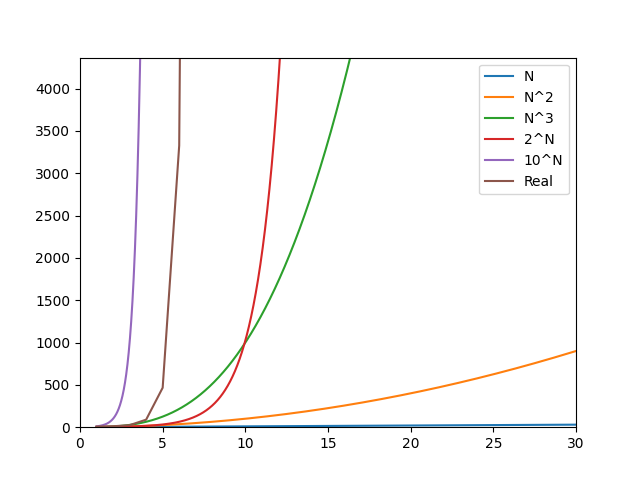
\includegraphics[scale=0.5]{normales.png}%
        \hspace{0.1\linewidth}%
        % Please, notice the use of an optional short caption.
        \caption[]{Tiempo vs Tamaño de entrada para la versión sin optimizar del algoritmo de coloreado de grafos.}
        \label{fig:res_normales}
    \end{figure}

    \begin{figure}[p]
        \centering
        % Please, notice the use of comments (%) to avoid extra space.
        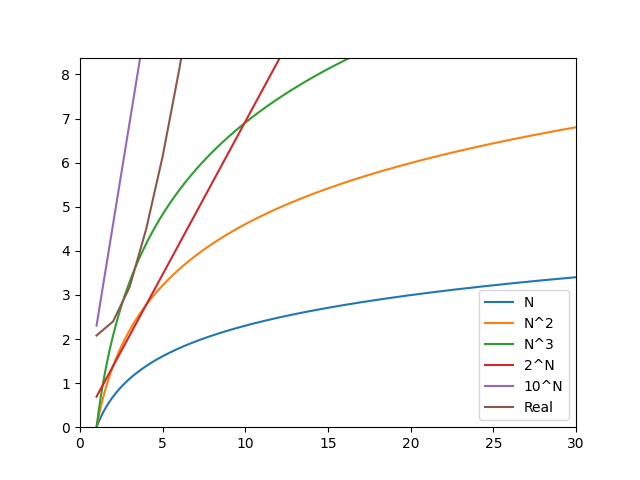
\includegraphics[scale=0.5]{normales_log.png}%
        \hspace{0.1\linewidth}%
        % Please, notice the use of an optional short caption.
        \caption[]{Logaritmo del tiempo vs Tamaño de entrada para la versión sin optimizar del algoritmo de coloreado de grafos.}
        \label{fig:res_normales_log}
    \end{figure}

    \begin{figure}[p]
        \centering
        % Please, notice the use of comments (%) to avoid extra space.
        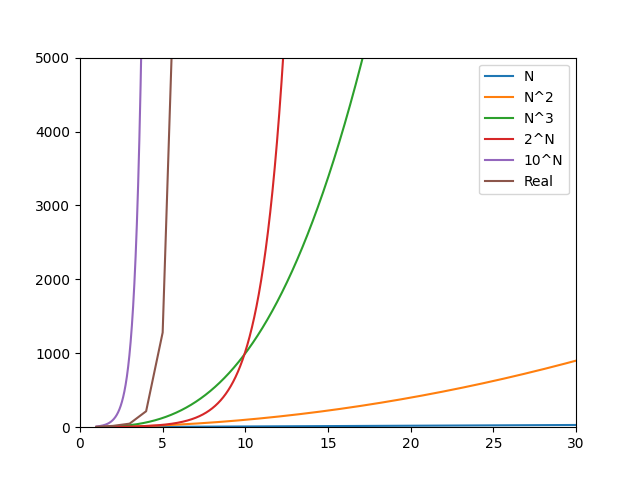
\includegraphics[scale=0.5]{optimizado.png}%
        \hspace{0.1\linewidth}%
        % Please, notice the use of an optional short caption.
        \caption[]{Tiempo vs Tamaño de entrada para la versión optimizada del algoritmo de coloreado de grafos.}
        \label{fig:res_optimizado}
    \end{figure}

    \begin{figure}[p]
        \centering
        % Please, notice the use of comments (%) to avoid extra space.
        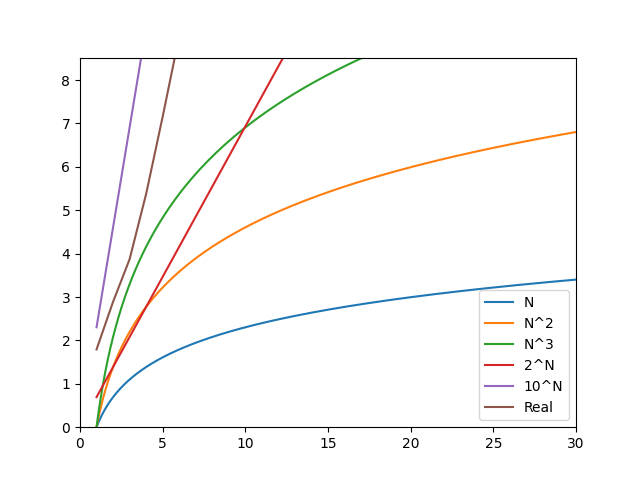
\includegraphics[scale=0.5]{optimizado_log.png}%
        \hspace{0.1\linewidth}%
        % Please, notice the use of an optional short caption.
        \caption[]{Logaritmo del tiempo vs Tamaño de entrada para la versión optimizada del algoritmo de coloreado de grafos.}
        \label{fig:res_optimizado_log}
    \end{figure}

    \clearpage

%%%% CONCLUSIONS %%%%%%%%%%%%%%%%%%%%%%%%%%%%%%%%%%%%%%%%%%%%%%%%%%%%%%%%%%%%%%%

    \section{Conclusions}
    \label{sec:conclusions}
    El algoritmo en pseudocódigo es fácil de entender una vez que lo miras con detenimiento aunque al principio puede costar un poco entenderlo. La implementación del mismo en \emph{C++} si que me ha ocasionado algunos problemas (especialmente al tratar con puntero), aunque he podido arreglar los fallos surgidos sin demasiada dificultad.
    \\
    En cuanto al generador de instancias del problema, con los números presentados en clase, es imposible obtener un grafo que no sea completo. Todas y cada una de las instancias generadas han creado conflictos con el resto de vértices del grado lo cuál ocasiona que el algoritmo esté siempre en el peor caso posible (tiene que recorrer un mayor número de nodos del árbol de búsqueda).
    \\
    También a la hora de calcular los tiempos de cada versión del algoritmo tuve problemas por la cantidad de tiempo que tomaba para valores de $N>12$. Es por eso que tuve que acotar los tamaños de entrada del algoritmo a un rango inferior para poder obtener tiempos suficientes con los que poder ver la forma aproximada de la función en una gráfica.
    \\
    Aunque todos los casos vistos han conducido a una búsqueda casi exhaustiva del árbol de búsqueda del problema, me ha ayudado a comprender mejor los problemas de este tipo de algoritmos que tienen que realizar búsquedas completas en su árbol de búsqueda y cómo hemos podido dar solución a un problema de la vida real (muy relacionado con otros tipos de problemas de otras áreas), reduciendo el problema a uno ya conocido y para el cuál tenemos un algoritmo que nos pueda proporcionar una solución.

    \clearpage

%%%%  REFEREroach NCES %%%%%%%%%%%%%%%%%%%%%%%%%%%%%%%%%%%%%%%%%%%%%%%%%%%%%%%%%%%%%%%%

%\section{References}
%\label{sec:references}


% Print the references collected in the first segment. No heading, as we have
% already included a numbered section, References, on their own.

%\printbibliography[segment=1,heading=none]


%%%%%%%%%%%%%%%%%%%%%%%%%%%%%%%%%%%%%%%%%%%%%%%%%%%%%%%%%%%%%%%%%%%%%%%%%%%%%%%%
%                                  APPENDICES                                  %
%%%%%%%%%%%%%%%%%%%%%%%%%%%%%%%%%%%%%%%%%%%%%%%%%%%%%%%%%%%%%%%%%%%%%%%%%%%%%%%%

%%%%%%%%%%%%%%%%%%%%%%%%%%%%%%%%%%%%%%%%%%%%%%%%%%%%%%%%%%%%%%%%%%%%%%%%%%%%%%%%
%                                 BACK MATTER                                  %
%%%%%%%%%%%%%%%%%%%%%%%%%%%%%%%%%%%%%%%%%%%%%%%%%%%%%%%%%%%%%%%%%%%%%%%%%%%%%%%%

% In standard classes, the following command is just markup (no visual effect).

% \backmatter

% Instead, we will start a new page after flushing floats.

    \cleardoublepage

%%%% BIBLIOGRAPHY %%%%%%%%%%%%%%%%%%%%%%%%%%%%%%%%%%%%%%%%%%%%%%%%%%%%%%%%%%%%%%

    \section*{Bibliography}
    \label{sec:bibliography}

% Provide some space between the text and the list of references. We can also
% use a small space (\smallskip), a medium one (\medskip), or simply omit it.

    \bigskip

% We can comment the following two lines and have just one section: the default
% section, 0. Previously defined segments would then refer to the default
% section and their numeric labels would match those in the following full list
% of references (the bibliography), instead of being independent.

    \endrefsection               % Enclose previous segments in the default section.
    \newrefsection               % Create a new section.

% Collect and print all the references in the current section.

    \nocite{*}
    \printbibliography[heading=none]

% With an explicit title:
%
% \printbibliography[title=Bibliography]

% With the default title in the table of contents:
%
% \printbibliography[heading=bibintoc]

\end{document}

%%%%%%%%%%%%%%%%%%%%%%%%%%%%%%%%%%%%%%%%%%%%%%%%%%%%%%%%%%%%%%%%%%%%%%%%%%%%%%%%
%
% Emacs related stuff.
%
% Emacs is an incredibly powerful programmable text editor. Please, find
% relevant information in the following links:
%
%     https://www.gnu.org/software/emacs/emacs.html
%     https://www.gnu.org/software/emacs/manual/emacs.html
%
% Emacs' local variables allow to configure Emacs on a per-file basis when a
% file is opened. The following lines are hardly needed, though they will
% not hurt:
%
%     coding: utf-8        ; Coding.
%     mode: latex          ; Major mode for LaTeX.
%     eval: (tex-pdf-mode) ; Minor mode for using PDFLaTeX.
%
% Emacs tries to guess the file encoding automatically. It can even peek the
% file's \usepackage[···]{inputenc} command, if any. The same with the major
% mode for editing LaTeX (latex-mode) and the minor mode for using PDF-TeX/LaTeX
% (tex-pdf-mode) from Emacs. AUCTeX is recommended to everyone willing to use
% Emacs as an integrated development environment for TeX, LaTeX, and
% derivatives.
%
% You may wish to force spell checking of the whole buffer when you finish
% editing your document, be it interactive (M-x ispell-buffer) or not (M-x
% flyspell-buffer).
%
%%%%%%%%%%%%%%%%%%%%%%%%%%%%%%%%%%%%%%%%%%%%%%%%%%%%%%%%%%%%%%%%%%%%%%%%%%%%%%%%

% Local variables:
% eval: (auto-fill-mode)             ; Automatic line breaking.
% fill-column: 80                    ; Last column before line breaking.
% ispell-local-dictionary: "british" ; Dictionary for spell checking.
% eval: (flyspell-mode)              ; Spell checking on the fly.
% End: